\section*{List of Symbols}
\label{sec:symbols}

\begin{table}[h!]
\centering
\small
\begin{tabular}{ll p{8cm}}
\toprule
\textbf{Symbol} & \textbf{Units} & \textbf{Description} \\
\midrule
\multicolumn{3}{l}{\textit{Nodal Degrees of Freedom (FEM Beam Elements)}} \\
$w$          & m   & Transverse (out-of-plane) bending displacement \\
$\phi$        & rad & Out-of-plane bending slope ($\partial w / \partial x$) \\
$\theta$     & rad & Torsion (twist) angle of the section \\
$\beta$      & rad & Flap deflection angle \\
\addlinespace
\multicolumn{3}{l}{\textit{Rigid-Body States \& Motion (Perturbations around Trim)}} \\
$P_x, P_y, P_z$ & m   & Rigid-body positions in Earth-fixed frame \\
$u, v, w$    & m/s & Body-axis translational velocities (longitudinal, lateral, heave) \\
$\phi, \theta, \psi$ & rad & Euler angles (roll, pitch, yaw) \\
$p, q, r$    & rad/s & Body rates (roll, pitch, yaw rate) \\
\addlinespace
\multicolumn{3}{l}{\textit{Aerodynamic \& Geometric Parameters}} \\
$\rho$       & kg/m$^3$ & Atmospheric density \\
$V$, \texttt{Vel} & m/s & Reference trim flight velocity ($V = 35$~m/s) \\
$\alpha_{\text{trim}}$ & rad & Trim angle of attack \\
$\alpha_{ht}, \beta_{vt}$ & rad & Local horizontal-tail angle of attack and vertical-tail sideslip angle \\
$\delta_e, \delta_r$ & rad & Elevator and rudder control surface deflections \\
$S_{ht}, S_{vt}$ & m$^2$ & Planform areas of the horizontal and vertical tails \\
$C_{L\alpha}, C_{L\beta}$ & rad$^{-1}$ & Lift-curve slopes of the respective aerodynamic surfaces \\
$C_{L\delta_e}, C_{L\delta_r}$ & rad$^{-1}$ & Control surface lift derivatives \\
$\boldsymbol{r}_{ht}, \boldsymbol{r}_{vt}$ & m & Position vectors from the center of gravity to the tail aerodynamic centers \\
$d_{rw}, d_{lw}$ & m & Chordwise moment arms from center of gravity to quarter-chord \\
$k_D$        & --- & Induced drag coefficient factor \\
$c$, \texttt{chord} & m & Mean aerodynamic chord length \\
\bottomrule
\end{tabular}
\end{table}

\newpage

\section{Flight Dynamic Model Implementation}
\label{sec:partB-implementation}

The full-aircraft flight dynamic model is assembled from three independently built pieces: the rigid-body equations of motion with the tail aerodynamics, the per-wing aeroelastic state space, and the coupling matrices that pass loads and motion between them. Two modules in the supporting code are left incomplete and must be filled before any free-flying configuration can be built. The first is the tail aerodynamic Jacobian \texttt{Get\_Aero\_Jacobian\_Tail}, where six derivatives are commented out and then used immediately, so the module raises a \texttt{NameError} on import. The second is the left-wing block of \texttt{Get\_Coupling\_Matrices}, where \texttt{R\_F\_lw} and \texttt{R\_M\_lw} are referenced but never defined. Both modules are imported when \texttt{main\_Aircraft\_Flight\_Dynamics.py} loads, so neither the rigid aircraft nor the flexible aircraft can be constructed until they are complete. This section explains why each missing term takes the form it does and how it is derived.

\subsection{Tail aerodynamic Jacobian}
\label{sec:partB-tail-jacobian}

The horizontal and vertical tails are treated as rigid bodies with quasi-steady strip aerodynamics. Writing $\boldsymbol{r}_{ht}=[r_{ht,x},0,r_{ht,z}]^{\top}$ and $\boldsymbol{r}_{vt}=[r_{vt,x},0,r_{vt,z}]^{\top}$ for the vectors from the centre of gravity to the two aerodynamic centres (the spanwise arm is zero because both centres lie in the symmetry plane), the body-frame tail force is
\begin{equation}
    \begin{bmatrix} F_x \\ F_y \\ F_z \end{bmatrix}_{\text{tail}}
    = \begin{bmatrix} -D_{ht} \\ 0 \\ -L_{ht} \end{bmatrix}
    + \begin{bmatrix} -D_{vt} \\ -L_{vt} \\ 0 \end{bmatrix},
    \label{eq:tail-force}
\end{equation}
with horizontal-tail lift $L_{ht}=\tfrac12\rho V^2 S_{ht}\,(C_{L\alpha}\alpha_{ht}+C_{L\delta_e}\delta_e)$ and vertical-tail lift $L_{vt}=\tfrac12\rho V^2 S_{vt}\,(C_{L\beta}\beta_{vt}+C_{L\delta_r}\delta_r)$. The Jacobian is the partial derivative of these loads with respect to the rigid-body perturbation states, evaluated at trim where $\beta_*=p_*=q_*=r_*=0$.

The key step is the chain rule through the local aerodynamic angles. The angle of attack seen by the horizontal tail and the sideslip seen by the vertical tail are, to first order,
\begin{equation}
    \alpha_{ht} = \frac{w - q\,r_{ht,x}}{V}, \qquad
    \beta_{vt}  = \frac{v - p\,r_{vt,z} + r\,r_{vt,x}}{V},
    \label{eq:tail-local-angles}
\end{equation}
so that $\partial\alpha_{ht}/\partial w = 1/V$, $\partial\alpha_{ht}/\partial q = -r_{ht,x}/V$, $\partial\beta_{vt}/\partial v = 1/V$, $\partial\beta_{vt}/\partial p = -r_{vt,z}/V$, and $\partial\beta_{vt}/\partial r = r_{vt,x}/V$. Each missing rate or control derivative is a load coefficient multiplied by one of these angle sensitivities. Because the rate derivatives share the factor $\tfrac12\rho V^2 S\,C_L$ already present in the corresponding velocity derivative, they can be written compactly as that velocity derivative scaled by the relevant moment arm, which is exactly the pattern the supplied $X$-row uses.

\paragraph{Side-force row.}
The given term is $Y_{v} = -\tfrac12\rho V S_{vt} C_{L\beta}$. The two missing rate derivatives follow from the $\beta_{vt}$ sensitivities above,
\begin{equation}
    Y_{p} = \frac{\partial F_y}{\partial p}
          = -r_{vt,z}\,Y_{v}, \qquad
    Y_{r} = \frac{\partial F_y}{\partial r}
          = r_{vt,x}\,Y_{v},
    \label{eq:tail-Y-rates}
\end{equation}
and the rudder derivative is the direct control sensitivity of the vertical-tail lift,
\begin{equation}
    Y_{\delta_r} = \frac{\partial F_y}{\partial \delta_r}
                 = -\tfrac12\rho V^2 S_{vt}\,C_{L\delta_r}.
    \label{eq:tail-Y-dr}
\end{equation}
In code these are \texttt{Y\_p\_T = Y\_v\_T*(-par['r\_cg\_vt'][2])}, \texttt{Y\_r\_T = Y\_v\_T*par['r\_cg\_vt'][0]} and \texttt{Y\_dr\_T = -0.5*rho*Vel**2*par['S\_Vtail']*par['Cl\_delta\_r']}, which mirror the form of the already-supplied \texttt{X\_p\_T} and \texttt{X\_r\_T}.

\paragraph{Normal-force row.}
The given term is $Z_{w} = -\tfrac12\rho V S_{ht} C_{L\alpha}$. The pitch-rate derivative uses the horizontal-tail arm and the elevator derivative is the direct control sensitivity of the horizontal-tail lift,
\begin{equation}
    Z_{q} = \frac{\partial F_z}{\partial q} = -r_{ht,x}\,Z_{w}, \qquad
    Z_{\delta_e} = \frac{\partial F_z}{\partial \delta_e}
                 = -\tfrac12\rho V^2 S_{ht}\,C_{L\delta_e}.
    \label{eq:tail-Z}
\end{equation}
In code, \texttt{Z\_q\_T = Z\_w\_T*(-par['r\_cg\_ht'][0])} and \texttt{Z\_de\_T = -0.5*rho*Vel**2*par['S\_Htail']*par['Cl\_delta\_e']}.

\paragraph{Pitching-moment row.}
The tail moments follow from $\boldsymbol{M}=\boldsymbol{r}\times\boldsymbol{F}$. With the spanwise arm zero, the three components reduce to $M_x=-r_z F_y$, $M_y=r_z F_x - r_x F_z$ and $M_z=r_x F_y$. The supplied roll and yaw rows, \texttt{L\_T = -par['r\_cg\_vt'][2]*Y\_T} and \texttt{N\_T = par['r\_cg\_vt'][0]*Y\_T}, are the $M_x$ and $M_z$ expressions applied to the vertical-tail side force. The missing pitching moment is the $M_y$ expression. It needs the drag contribution split between the two tails, because each acts at its own vertical arm, which is why the module pre-computes \texttt{X\_T\_ht} and \texttt{X\_T\_vt} separately:
\begin{equation}
    M_y = r_{ht,z}\,F_x^{ht} + r_{vt,z}\,F_x^{vt} - r_{ht,x}\,F_z .
    \label{eq:tail-M}
\end{equation}
In code this is \texttt{M\_T = par['r\_cg\_ht'][2]*np.array(X\_T\_ht) + par['r\_cg\_vt'][2]*np.array(X\_T\_vt) - par['r\_cg\_ht'][0]*Z\_T}. With these six terms defined the stacked Jacobian \texttt{Jco\_Tail} assembles without error and reproduces the structure of the guideline, namely a force block driving $[u,v,w]$ and $[p,q,r]$ with the elevator and rudder columns, and a moment block with the matching sparsity.

\subsection{Wing coupling matrices}
\label{sec:partB-coupling}

The coupling stage transfers the wing root loads into the rigid-body forcing and the rigid-body motion into the local strip angle of attack. The angle-of-attack maps \texttt{R\_AOA\_rw} and \texttt{R\_AOA\_lw} are already provided; the remaining task is the left-wing load-transfer block \texttt{R\_FM\_lw}, built from a force part \texttt{R\_F\_lw} and a moment part \texttt{R\_M\_lw} that stack into the $[\,0,\,\Delta F_y,\,0,\,\Delta M\,]$ slots of the twelve-row rigid-body forcing vector.

The right-wing block is the template. Its force part sends the wing lift to a negative body-$z$ force and to an induced-drag increment along body-$x$, and its moment part sends the root bending moment to roll, and the lift arm and root torsion to pitch:
\begin{equation}
    \mathbf{R}_{F,rw} =
    \begin{bmatrix} -2 k_D C_{L\alpha}\alpha_{\text{trim}} & 0 & 0 \\ 0 & 0 & 0 \\ -1 & 0 & 0 \end{bmatrix},
    \qquad
    \mathbf{R}_{M,rw} =
    \begin{bmatrix} 0 & -1 & 0 \\ d_{rw} & 0 & 1 \\ 0 & 0 & 0 \end{bmatrix},
    \label{eq:Rrw}
\end{equation}
where $d_{rw}=r_{cg,rw,x}-0.25\,c$ is the chordwise arm from the centre of gravity to the quarter-chord, and the three columns correspond to the wing outputs $[\text{lift}, \text{bending}, \text{torsion}]$.

The left wing follows from the mirror rule. The two half-wings are geometric mirror images about the body $x$-$z$ plane, so body-frame force directions are identical on both sides: lift still acts up and induced drag still acts aft. The force block is therefore unchanged,
\begin{equation}
    \mathbf{R}_{F,lw} = \mathbf{R}_{F,rw}.
    \label{eq:Rflw}
\end{equation}
The moment transfer is where the sides differ. The roll contribution flips sign, because a root bending moment on the left wing rolls the aircraft the opposite way to the same moment on the right wing; the pitch contribution keeps its sign, because pitch acts through the side-independent chordwise arm. Flipping only the roll row of $\mathbf{R}_{M,rw}$ gives
\begin{equation}
    \mathbf{R}_{M,lw} =
    \begin{bmatrix} 0 & +1 & 0 \\ d_{lw} & 0 & 1 \\ 0 & 0 & 0 \end{bmatrix},
    \qquad d_{lw}=r_{cg,lw,x}-0.25\,c .
    \label{eq:Rmlw}
\end{equation}
By symmetry $d_{lw}=d_{rw}$, but the left-wing centre-of-gravity coordinate \texttt{par['r\_cg\_lw']} is used so the construction stays explicit. In code the block is

\begin{verbatim}
R_F_lw = np.zeros((3, 3))
R_F_lw[0, 0] = -2 * par['kD'] * par['Clalpha_W'] * par['alpha_trim']
R_F_lw[2, 0] = -1

R_M_lw = np.zeros((3, 3))
R_M_lw[0, 1] = 1
arm_cg_ec_lw = par['r_cg_lw'][0, 0] - 0.25 * par['chord'][0]
R_M_lw[1, 0] = arm_cg_ec_lw
R_M_lw[1, 2] = 1
\end{verbatim}

The only change from the right-wing block is the sign of the bending-to-roll entry, \texttt{R\_M\_lw[0,1] = 1} against \texttt{R\_M\_rw[0,1] = -1}. This single sign flip carries the left-right asymmetry that produces the rolling response to an asymmetric flap input.

With both modules complete, \texttt{Get\_EQM\_Coupled\_Flight\_Dynamics} assembles the block system $[[\,\text{rigid}, \text{rw}_{\text{out}}, \text{lw}_{\text{out}}\,], [\,\text{rw}_{\text{in}}, A_{ww}, 0\,], [\,\text{lw}_{\text{in}}, 0, A_{ww}\,]]$, and the rigid aircraft (40 states) and flexible aircraft (180 states) can both be built and analysed.

\subsection{Eigenvalue analysis}
\label{sec:partB-eigenvalues}

The two configurations are compared through the eigenvalues of their system matrices $A_{\text{Fdyn}}$: the rigid aircraft with quasi-steady aerodynamics (40 states) and the flexible aircraft with unsteady aerodynamics (180 states). Figure~\ref{fig:partB-eigenvalues} plots both spectra in the complex plane, with the full pole landscape on the left and a zoom on the near-origin flight-dynamics region on the right.

\paragraph{Mode identification.}
The named rigid-body modes are not assigned from their position in the plane but from the eigenvectors, which makes the labels defensible even when poles lie close together. For each eigenvalue $\lambda_i$ with eigenvector $\boldsymbol{v}_i$, a normalised participation is formed for every state $j$,
\begin{equation}
    p_{ij} = \frac{|v_{ij}|}{\sum_k |v_{kj}|},
    \label{eq:participation}
\end{equation}
and the contributions of the six body-axis velocity and rate states $[u,v,w,p,q,r]$ are examined. A mode is a rigid-body mode when these dominate its eigenvector; the kinematic integrators (the positions $P_x,P_y,P_z$ and heading $\psi$) appear as eigenvalues at the origin and are excluded. The classical modes are then distinguished by which body states dominate: the \emph{short-period} by heave and pitch rate $(w,q)$, the \emph{phugoid} by axial velocity $u$, the \emph{Dutch roll} by sideslip and yaw rate $(v,r)$, the \emph{roll subsidence} by a fast real root in roll rate $p$, and the \emph{spiral} by a slow real root in bank and heading. The same procedure applied to the flexible aircraft distinguishes the rigid-body modes from the aeroelastic (wing-bending and torsion) and aerodynamic-lag modes that fill the rest of the spectrum.

\begin{figure}[htbp]
    \centering
    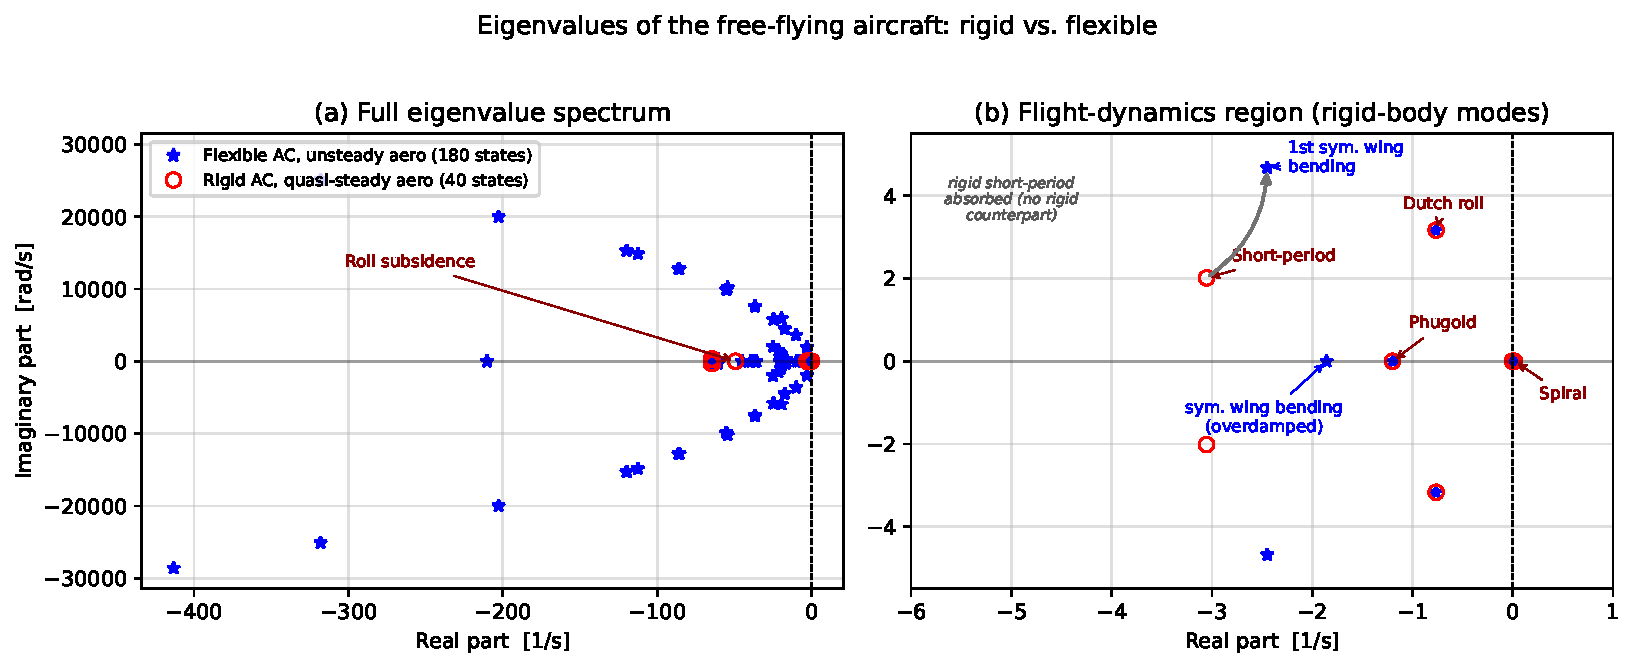
\includegraphics[width=\textwidth]{figures/partB_aircraft_eigenvalues.pdf}
    \caption{Eigenvalues of the free-flying aircraft: rigid aircraft with quasi-steady aerodynamics (red circles, 40 states) and flexible aircraft with unsteady aerodynamics (blue stars, 180 states). Panel~(a) shows the full spectrum; panel~(b) zooms on the flight-dynamics region. The rigid-body modes are labelled in dark red on the rigid aircraft as reference; the two flexible symmetric wing-bending modes that fall in this region (an oscillatory pair and an overdamped real root) are labelled in blue. The grey arrow indicates that the rigid short-period oscillation has no rigid-body counterpart in the flexible aircraft: its heave/pitch content is absorbed into the symmetric wing-bending modes.}
    \label{fig:partB-eigenvalues}
\end{figure}

\paragraph{Rigid-aircraft modes and stability.}
The rigid aircraft exhibits the five expected modes. The short-period is a well-damped oscillation at $\lambda=-3.05\pm2.01i$ ($\zeta=0.84$), the Dutch roll a more lightly damped oscillation at $-0.76\pm3.17i$ ($\zeta=0.24$), and the roll subsidence a fast real root at $-49.3$. The phugoid is \emph{overdamped}, appearing as a real root at $-1.20$ rather than the usual lightly damped oscillation. The spiral is the only unstable mode, a slow real root at $+0.018$; the aircraft is therefore statically/dynamically stable in every mode except a benign spiral divergence whose time-to-double is long enough to be of little practical concern for this glider.

\paragraph{Effect of flexibility.}
Table~\ref{tab:partB-modes} compares the modes between the two aircraft. The pattern is physically clean: flexibility most disturbs exactly the modes whose rigid-body motion couples into wing bending, and barely touches those that do not.
\begin{table}[htbp]
    \centering
    \caption{Rigid-body modes of the rigid and flexible aircraft, identified from the eigenvectors via Eq.~\eqref{eq:participation}.}
    \label{tab:partB-modes}
    \begin{tabular}{l l l l}
    \hline
    Mode & Rigid AC & Flexible AC & Effect of flexibility \\
    \hline
    Short-period    & $-3.05\pm2.01i$ ($\zeta{=}0.84$) & no rigid-body mode            & dissolved into sym.\ bending \\
    Phugoid         & $-1.20$ (overdamped)             & $-1.19$ (overdamped)          & negligible \\
    Dutch roll      & $-0.76\pm3.17i$ ($\zeta{=}0.24$) & $-0.77\pm3.17i$ ($\zeta{=}0.24$) & negligible \\
    Roll subsidence & $-49.3$                          & $\approx-8.3$ (smeared)       & damping strongly reduced \\
    Spiral          & $+0.018$ (unstable)              & $+0.018$ (unstable)           & negligible \\
    \hline
    \end{tabular}
\end{table}

The \emph{short-period} has no rigid-body counterpart in the flexible aircraft. In the rigid model it carries a large heave participation ($p_{ij}=0.58$ in $w$); in the flexible model no eigenvalue retains more than $p_{ij}=0.01$ of rigid pitch rate. The heave/pitch motion is instead absorbed into the symmetric wing-bending modes, which appear as a real root near $-1.86$ and an oscillatory pair near $-2.45\pm4.68i$ (both left--right symmetric, dominated by the nodal bending DOFs $w$ and $\phi$ with negligible torsion). This coupling, indicated by the arrow in Figure~\ref{fig:partB-eigenvalues}(b), is the most prominent new aeroelastic feature. The \emph{roll subsidence} is similarly affected: its clean rigid pole at $-49.3$ gives way to a roll-rate participation that is smeared across several aeroelastic poles, the most roll-dominant lying near $-8.3$, so the effective roll damping drops sharply because the wing twists and bends under roll rate. By contrast the \emph{Dutch roll}, \emph{phugoid} and \emph{spiral} are essentially unchanged, because they are dominated by sideslip, yaw and slow speed/heading motion that couples only weakly into wing bending. The spiral instability persists with the same growth rate, so flexibility does not alter the aircraft's overall stability verdict, only the character of its longitudinal and roll dynamics. The remainder of the flexible spectrum, visible in Figure~\ref{fig:partB-eigenvalues}(a), consists of higher-frequency wing-bending and torsion modes and the heavily damped aerodynamic-lag poles introduced by the unsteady aerodynamics, none of which has a rigid-aircraft analogue.
